\section{Risk Management and Mitigation}
\label{sec:monitoring}

\subsection{Attack Surfaces}

\begin{figure*}[t]
  \centering
  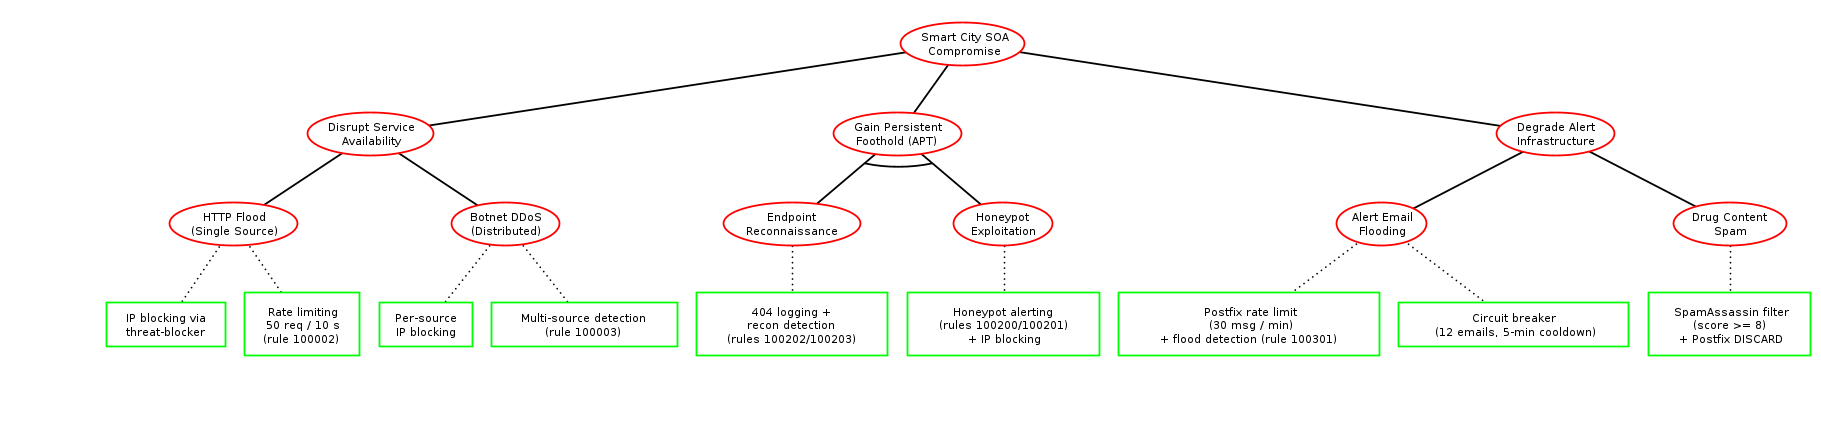
\includegraphics[width=\textwidth]{images/smart_city_attacktree}
  \caption{Attack-Defense Tree for the Smart City SOA. Red ovals represent attack nodes;
  green rectangles represent countermeasures.}
  \label{fig:attacktree}
\end{figure*}

Seven attack surfaces are identified in the Smart City SOA. Four are addressed by
the threat classes in Sections~5 through~9; three are recorded as residual risks
out of scope for the current implementation.

\begin{itemize}[leftmargin=*]
  \item \textbf{Public HTTP layer:} the ops portal accepts
        unauthenticated operator traffic and is reachable from outside the VM.
        A single high-rate source exploiting this interface constitutes a DoS
        threat. A coordinated set of sources acting in concert constitutes a
        DDoS threat. Neither attack requires application-level knowledge.
  \item \textbf{Inter-service API layer:} service-to-service calls are
        authenticated via the \texttt{x-internal-token} header, but that token
        is reachable through the honeypot endpoints on zone aggregators. A token
        obtained through endpoint enumeration enables impersonation of any
        internal service. This is a multi-stage surface, corresponding to the
        APT threat class. The conjunctive structure of that branch in
        Figure~\ref{fig:attacktree} reflects the two-phase dependency.
  \item \textbf{Mail delivery path:} two independent surfaces exist on the mail
        channel. The alert service generates outbound notifications whose volume
        is bounded only by a circuit breaker, exposing the system to alert
        flooding. The Postfix relay on port 25 accepts inbound mail without
        content filtering at the transport layer, exposing the system to
        drug-content spam. Each maps to a distinct threat class.
  \item \textbf{Observability and logging path:} Wazuh ingests logs from a
        shared Incus bind-mount. A compromised container writing malformed JSON
        to that volume could disrupt rule processing. This surface is not
        addressed in the current implementation and is recorded as a residual
        risk.
  \item \textbf{Zone aggregator sensor endpoints:} zone aggregators are
        internal edge services, but ports 5100-5102 are externally mapped in
        the lab deployment to allow the PoC scripts to reach the honeypot
        endpoints. This exposes the sensor ingestion endpoints directly: an
        attacker could POST fabricated readings, corrupting stored data and
        triggering false threshold alerts without touching the honeypot. In a
        production deployment, zone aggregators should reside on an internal
        network segment reachable only by the ingestion and analytics services.
        This surface is recorded as a residual risk.
  \item \textbf{Service registry:} the service registry is
        unauthenticated in the current implementation. An attacker with network
        access could enumerate the full service topology or register a rogue
        service, poisoning discovery for legitimate callers. This surface is
        recorded as a residual risk.
  \item \textbf{Monitoring stack:} Prometheus and Grafana
      are reachable externally in the current deployment. These
        endpoints expose detection thresholds, per-rule hit counters, and service
        topology, allowing an attacker to calibrate traffic to remain below
        detection limits. In production, the monitoring stack should be placed
        behind an authenticated reverse proxy with no external port binding.
        This surface is recorded as a residual risk.
\end{itemize}

\subsection{Attack and Defense Trees}

Risk management in this platform is structured around three layers: continuous
observability through Prometheus and Grafana, event-driven intrusion detection through
the Wazuh SIEM, and automated active response through a custom threat-blocker service.
Figure~\ref{fig:attacktree} presents the Attack-Defense Tree for the four surfaces
that are actively exploited and defended in this project.

The root goal, \emph{Smart City SOA Compromise}, branches into three disjunctive
sub-goals corresponding to the three threat classes addressed. The
\emph{Disrupt Service Availability} branch is disjunctive: a single-source HTTP
flood and a distributed botnet DDoS are independent attack paths, each defended by
rate limiting and IP blocking. The \emph{Gain Persistent Foothold} branch is
conjunctive: both endpoint reconnaissance and honeypot exploitation must succeed,
so blocking either phase defeats the full chain. The
\emph{Degrade Alert Infrastructure} branch is disjunctive: alert email flooding
and drug content spam are independent, each requiring its own defence.

\subsection{Large-Scale System Monitoring}

Prometheus scrapes all services via a pull-based model at a 15-second global interval,
reduced to 5 seconds for the ops portal and the Wazuh exporter to minimise detection
latency on high-rate events.
Each service exposes a \texttt{/metrics} endpoint with counters for HTTP requests,
alert emails, spam events, and Wazuh rule hits. The Wazuh exporter bridges the SIEM
to Prometheus by tailing \texttt{alerts.json} and incrementing per-rule counters,
allowing Grafana to display detection events alongside service-level metrics on a
unified dashboard. Counters are pre-seeded at startup to avoid cold-start blind spots
on the first scrape interval.

Wazuh ingests structured JSON logs written by all services to a shared volume. Thirteen
custom rules are defined across four threat classes, using frequency-based
(\texttt{<frequency>}) and cross-source correlation (\texttt{<different\_field>})
primitives. Each rule that confirms a threat triggers an active response: Wazuh's
execution daemon invokes a shell script that sends an HTTP POST request to the
threat-blocker service, which applies a DROP rule in the \texttt{DOCKER-USER}
iptables chain. This chain intercepts DNAT-forwarded traffic before it reaches service
processes, correctly blocking traffic regardless of Docker's NAT rewriting. Blocked
addresses are automatically removed after 300 seconds.
